\documentclass[graphics]{beamer}

\usepackage{graphicx}
\usepackage{verbatim}
\usepackage{wrapfig}
\useoutertheme{shadow}
%\usecolortheme{orchid}
\usecolortheme{seahorse}


% math commands
\newcommand{\be}{\begin{eqnarray}}
\newcommand{\ee}{\end{eqnarray}}
\newcommand{\beq}{\begin{equation}}
\newcommand{\eeq}{\end{equation}}
\def\simless{\mathbin{\lower 3pt\hbox
      {$\rlap{\raise 5pt\hbox{$\char'074$}}\mathchar"7218$}}}
\def\simgreat{\mathbin{\lower 3pt\hbox
      {$\rlap{\raise 5pt\hbox{$\char'076$}}\mathchar"7218$}}} %> or of order

% variables

\def\toonscale{0.45}
\def\mboxy#1{\mbox{\small #1}}


\begin{comment}
\AtBeginSection[]{
  \frame{
    \frametitle{Outline}
    \tableofcontents[currentsection]
  }
}
\end{comment}

\title{Parity (violation) of the PTA gravitational wave background
}
%\subtitle{interim update}
\author[U. Pen]{Anna Tsai, Dylan Jow, Ue-Li Pen
}
\date{June 3, 2024}


\begin{document}

%\section*{Introduction}
\section{Lenses}

\begin{comment}
  \subsection{Outline}

  \frame{
    \frametitle{Outline}
    \tableofcontents
  }
\end{comment}

\frame{\maketitle}




  \frame{
    \frametitle{Pulsar Timing Arrays}
    \begin{itemize}
        \item first evidence of signal (nanoGrav+2023)
        \item due to supermassive black holes, or primordial
        \item polarized (L/R)?
    \end{itemize}
  }


  \frame{

    \frametitle{Is isotropic polarization detectable?}
   \begin{itemize}
        \item Boyle/ULP 2012+, Roebber+2017
        \item no-go theorems: Belgacem/Kamionkowski 2020, Kato/Soda 2016
        \item real timing residuals map to complex frequency residuals
        \item what correlations are allowed between complex fields on
          a sphere? 
        \item $\tau(\omega,\theta,\phi)=u(\theta,\phi)+i v(\theta,\phi)$
        \item CF CMB tensor mode helicity (Masui+2017): curved sky effects
    \end{itemize}
  }

  \frame{
    \frametitle{PTA redshift maps}
\vspace{-0.25in}
\begin{center}
%\hspace{-0.5in}
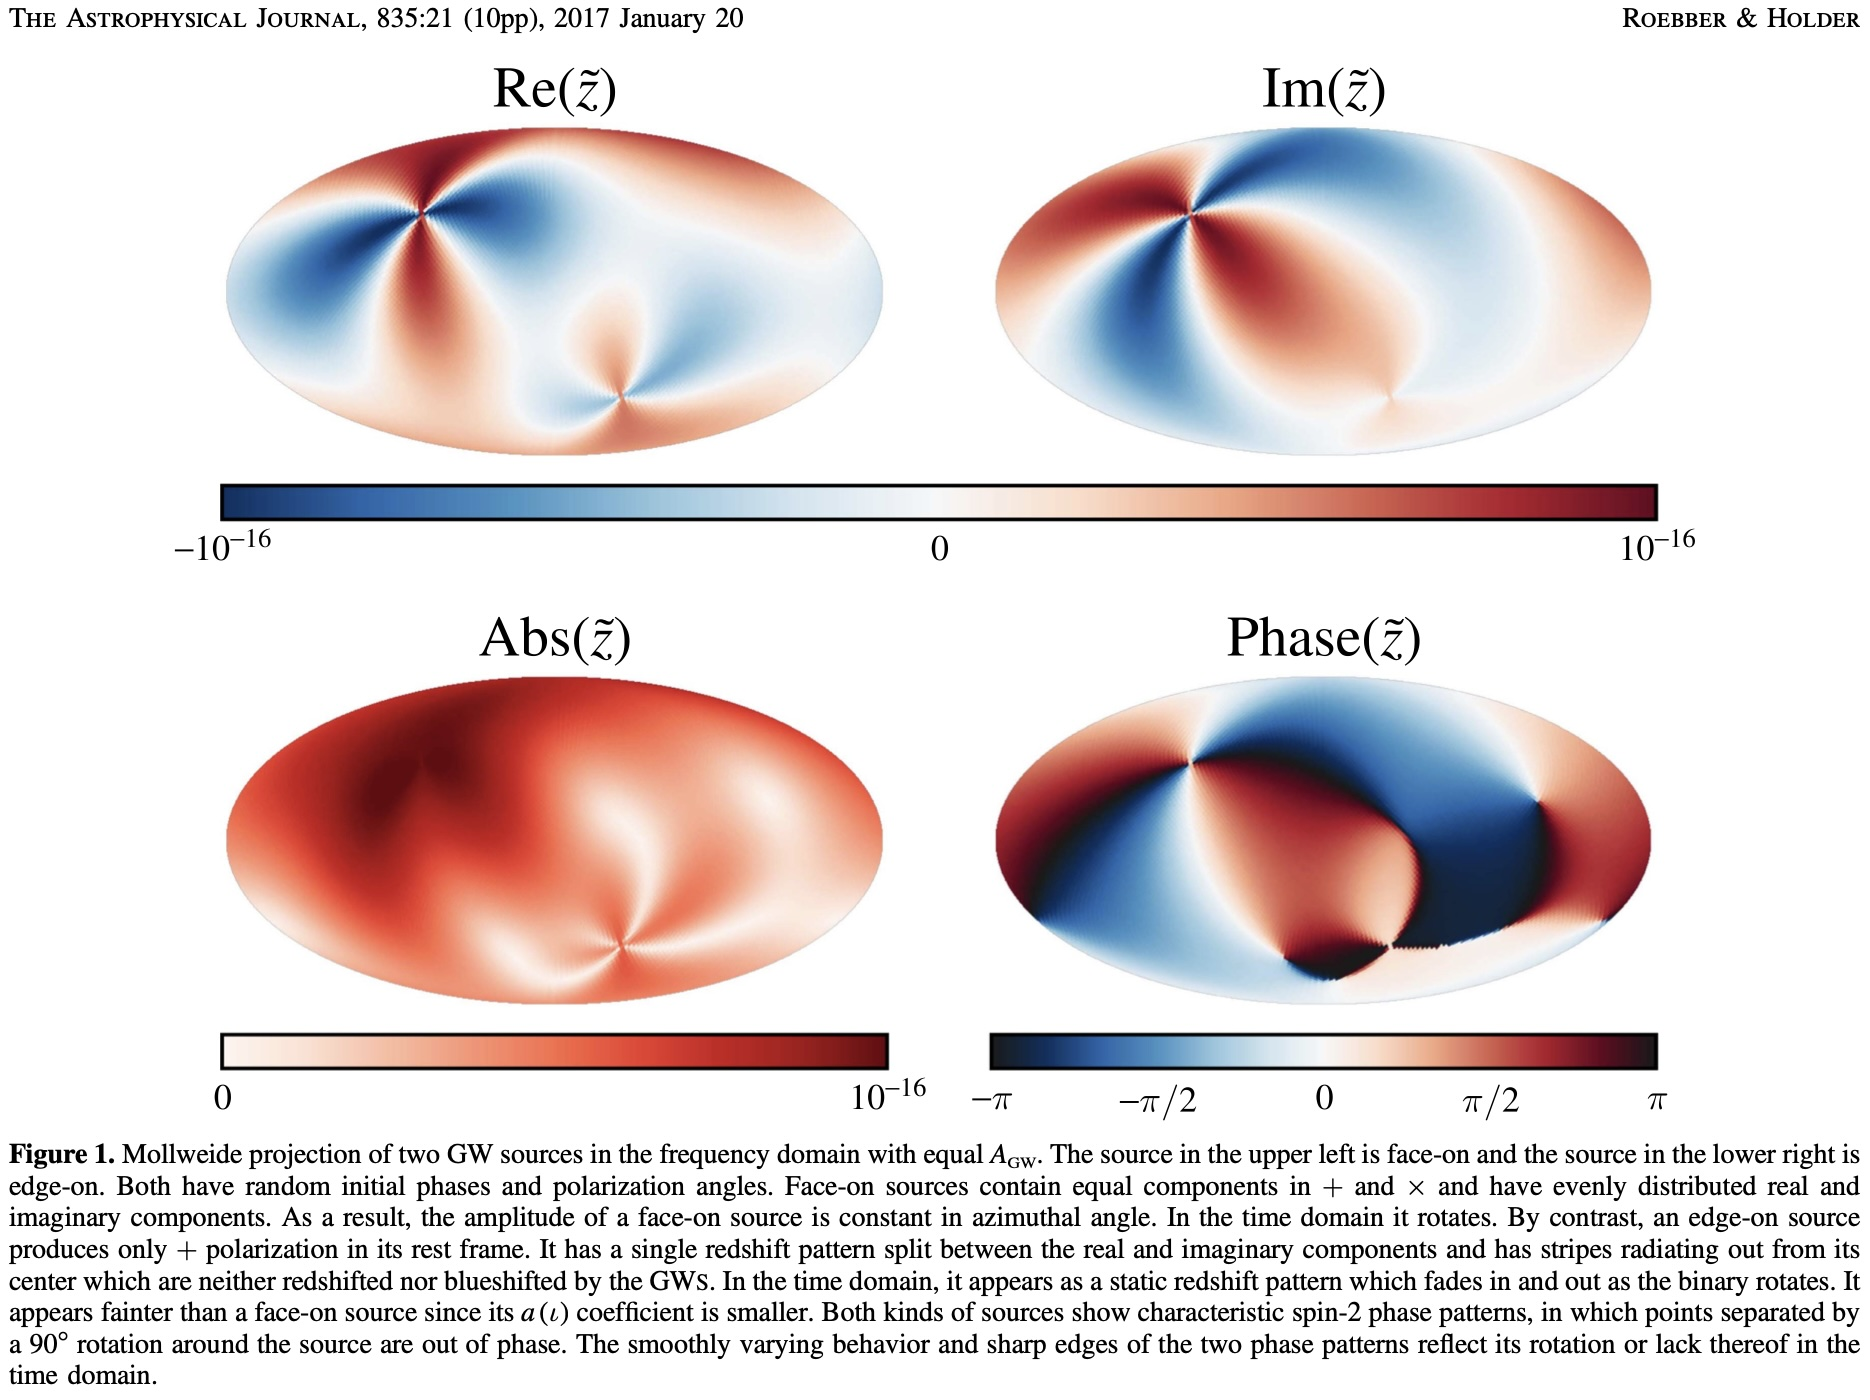
\includegraphics[width=4.5in]{Figures/RH17.jpg}
\end{center}
  }


  \frame{
    \frametitle{Subtle but strong}
   \begin{itemize}
        \item $\chi \equiv \nabla u \times \nabla v$
        \item $\bar{\chi}=\int \chi d\Omega = -3$
        \item violates Fubini theorem
    \end{itemize}
  }

  \frame{

    \frametitle{3/6 point quadratic?}
   \begin{itemize}
        \item $\chi$ is explicitly quadratic in timing residuals
        \item gradient requires 3 pulsars
        \item two effects of opposite sign: finite pulsar distance
          (for pairs separation $<1$ degree),
          curved sky.
        \item Polarized extension of Hellings-Downs curve using pulsar
          triplets
        \item not reducable to pair statistics: breakdown of
          integration by parts (Fubini), and non-commutation of covariant derivatives on sphere
    \end{itemize}
  }


  \frame{
    \frametitle{Chiral correlation}
\vspace{-0.5in}
\begin{center}
%\hspace{-0.5in}
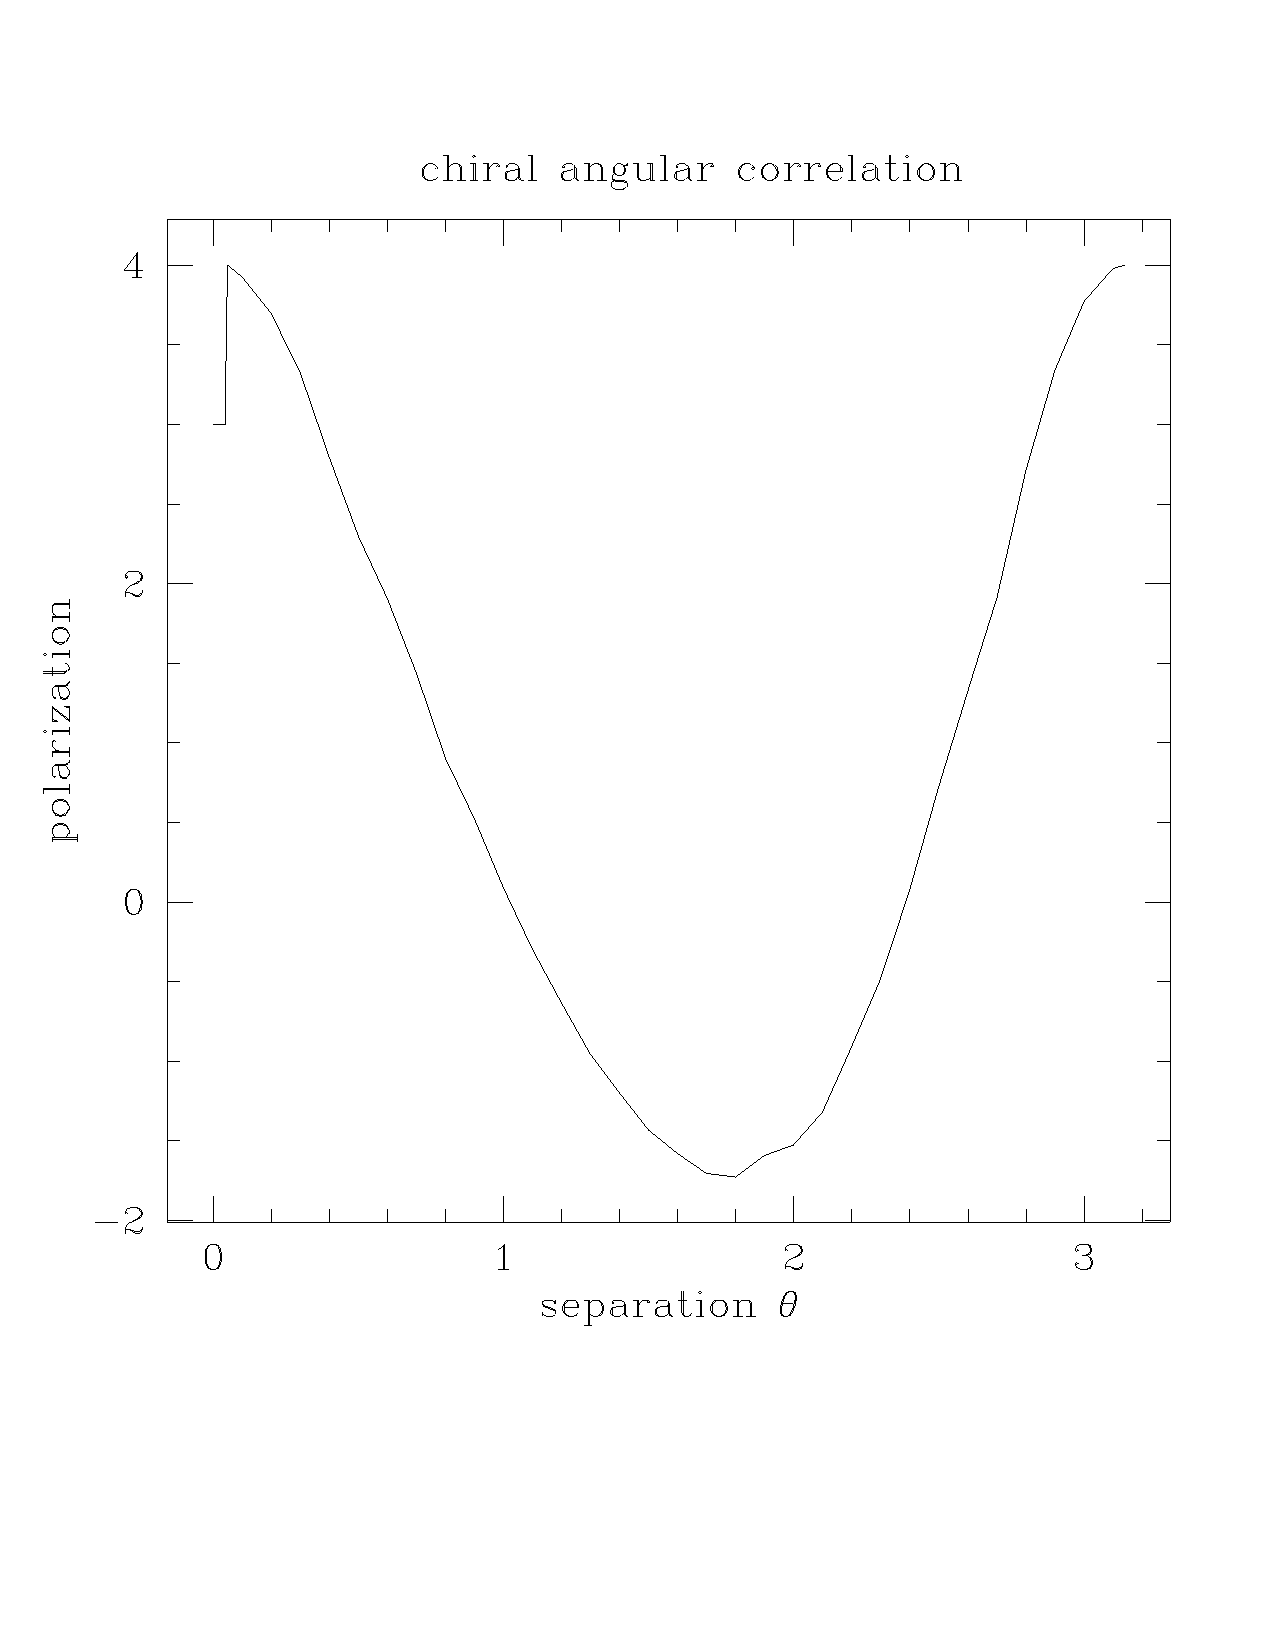
\includegraphics[width=3.2in]{Figures/corr.pdf}
\end{center}
  }


  \frame{

    \frametitle{Data Analysis}
   \begin{itemize}
        \item each pair of pulsars defines a gradient component
        \item two distinct gradient components needed for cross
          product
        \item signal dominated by widely separated triplets
        \item convenient analysis with Wirtinger derivatives
    \end{itemize}
  }



  \frame{
%\vspace{-0.5in}
    \frametitle{Summary}
    \begin{itemize}
    \item additional correlation information in PTA data
    \item incorrect PTA polarization literature
    \item quadratic estimator requires more than 2 points on a sphere!
     \item finite SMBH population always chiral!
     \item access to primordial symmetries, birefringent propagation
    \end{itemize}
  }

\end{document}
